\chapter{Tour to Dart Programming Language}

\section{Language sample}
\subsection{Hello World}


\begin{lstlisting}[language=C]
	
void main() {
	print('Hello, World!');
}
\end{lstlisting}
%\lstinputlisting[language=Python,style=mystyle, %caption=Factorial Program, %label=factorial.py]{code/factorial.py}

\section{Comments}
\subsection{Single Line Comments}
\begin{lstlisting}[language=C]
// This is a single line comment.
\end{lstlisting}
\subsection{Multi-Line Comments}
\begin{lstlisting}[language=C]
/* This is a multi-line comment.*/
\end{lstlisting}
\section{Return Type}
\textbf{void}: A special type that indicates a value that's never used. Functions like printInteger() and main() that don't explicitly return a value have the void return type.\\\\
\textbf{int}: It indicates that function will return integer value.\\\\
Similarly, with the String, Bool Return type etc.

\section{Declaring variables}
\textbf{var}: A way to declare a variable without specifying its type. The type of this variable (int) is determined by its initial value .
\begin{lstlisting}[language=C]
	var name = 'Bob';
\end{lstlisting}

Variables store references. The variable called name contains a reference to a String object with a value of "Bob".

The type of the name variable is inferred to be String, but you can change that type by specifying it. If an object isn't restricted to a single type, specify the Object type (or dynamic if necessary).
\begin{lstlisting}[language=C]
	Object name = 'Bob';
\end{lstlisting}

Another option is to explicitly declare the type that would be inferred:

\begin{lstlisting}[language=C]
	String name = 'Bob';
\end{lstlisting}

\section{Default value}
Uninitialized variables that have a nullable type have an initial value of null. (If you haven't opted into null safety, then every variable has a nullable type.) Even variables with numeric types are initially null, because numbers-like everything else in Dart-are objects.
\begin{lstlisting}[language=C]
	int? lineCount;
\end{lstlisting}

If you enable null safety, then you must initialize the values of non-nullable variables before you use them:

\begin{lstlisting}[language=C]
	int lineCount = 0;
\end{lstlisting}
You don't have to initialize a local variable where it's declared, but you do need to assign it a value before it's used.
\section{Assert Statements}
As a programmer, it is very necessary to make an errorless code is very necessary and to find the error is very difficult in a big program. Dart provides the programmer with assert statements to check for the error. The assert statement is a useful tool to debug the code and it uses boolean condition for testing. If the boolean expression in assert statement is true then the code continues to execute, but if it returns false then the code ends with Assertion.\\
\textbf{Syntax}: 
\begin{lstlisting}[language=C]
	assert(condition);
\end{lstlisting}
It must be noted that if you want to use assert then you have to enable it while execution as it can only be used in the development mode and not in productive mode. If it is not enabled then it will be simply be ignored while execution.
\\Enable the assert while executing a dart file via cmd as:

\begin{lstlisting}[language=C]
	dart --enable-asserts file_name.dart
\end{lstlisting}

\section{Late variables}
If you're sure that a variable is set before it's used, but Dart disagrees, you can fix the error by marking the variable as late:
\begin{lstlisting}[language=C]
	late String description;
	
	void main() {
		description = 'Feijoada!';
		print(description);
	}
\end{lstlisting}
\textbf{Warning}:  If you fail to initialize a late variable, a runtime error occurs when the variable is used.
 \\If you fail to initialize a late variable, a runtime error occurs when the variable is used.
 \\When you mark a variable as late but initialize it at its declaration, then the initializer runs the first time the variable is used. This lazy initialization is handy in a couple of cases:
\begin{itemize}
	\item The variable might not be needed, and initializing it is costly.
	\item You're initializing an instance variable, and its initializer needs access to this.
\end{itemize}

In the following example, if the temperature variable is never used, then the expensive readThermometer() function is never called:
\begin{lstlisting}[language=C]
	// This is the program's only call to _readThermometer().
	late String temperature = readThermometer(); // Lazily initialized.
\end{lstlisting}
\section{Final and const}
If you never intend to change a variable, use final or const, either instead of var or in addition to a type. A final variable can be set only once; a const variable is a compile-time constant. (Const variables are implicitly final.)
\\Instance variables can be final but not const.
\\\\Here's an example of creating and setting a final variable:
\begin{lstlisting}[language=C]
	final name = 'Bob'; // Without a type annotation
	final String nickname = 'Bobby';
	name = 'Alice'; // Error: a final variable can only be set once.
\end{lstlisting}

Use const for variables that you want to be compile-time constants. If the const variable is at the class level, mark it static const. Where you declare the variable, set the value to a compile-time constant such as a number or string literal, a const variable, or the result of an arithmetic operation on constant numbers:

\begin{lstlisting}[language=C]
	const bar = 1000000; // Unit of pressure (dynes/cm2)
	const double atm = 1.01325 * bar; // Standard atmosphere
\end{lstlisting}
You can change the value of a non-final, non-const variable, even if it used to have a const value:
\begin{lstlisting}[language=C]
	foo = [1, 2, 3]; // Was const []
\end{lstlisting}
\section{Built-in types}
The Dart language has special support for the following:
\begin{itemize}
\item Numbers (int, double)
\item Strings (String)
\item Booleans (bool)
\item Lists (List, also known as arrays)
\item Sets (Set)
\item Maps (Map)
\item Runes (Runes; often replaced by the characters API)
\item Symbols (Symbol)
\item The value null (Null)
\end{itemize}
This support includes the ability to create objects using literals. For example, 'this is a string' is a string literal, and true is a boolean literal.

Because every variable in Dart refers to an object—an instance of a class—you can usually use constructors to initialize variables. Some of the built-in types have their own constructors. For example, you can use the Map() constructor to create a map.
\subsection{Numbers}
\begin{itemize}
	\item int: Integer values no larger than 64 bits, depending on the platform.
	\item double: 64-bit (double-precision) floating-point numbers, as specified by the IEEE 754 standard.
	\item Strings: A Dart string (String object) holds a sequence of UTF-16 code units. You can use either single or double quotes to create a string:
	\begin{lstlisting}[language=C]
		var s1 = 'Single quotes work well for string literals.';
		var s2 = "Double quotes work just as well.";
		var s3 = 'It\'s easy to escape the string delimiter.';
		var s4 = "It's even easier to use the other delimiter.";
	\end{lstlisting}
You can put the value of an expression inside a string by using 
\begin{lstlisting}[language=C]
	${expression}
\end{lstlisting}

If the expression is an identifier, you can skip the 
\begin{lstlisting}[language=C]
	{}
\end{lstlisting}
To get the string corresponding to an object, Dart calls the object's toString() method.

\begin{lstlisting}[language=C]
	var s = 'string interpolation';
	
	assert('Dart has $s, which is very handy.' ==
	'Dart has string interpolation, '
	'which is very handy.');
	assert('That deserves all caps. '
	'${s.toUpperCase()} is very handy!' ==
	'That deserves all caps. '
	'STRING INTERPOLATION is very handy!');
\end{lstlisting}
 Note: The == operator tests whether two objects are equivalent. Two strings are equivalent if they contain the same sequence of code units.
 
 You can concatenate strings using adjacent string literals or the + operator:
 \begin{lstlisting}[language=C]
 	var s1 = 'String '
 	'concatenation'
 	" works even over line breaks.";
 	assert(s1 ==
 	'String concatenation works even over '
 	'line breaks.');
 	
 	var s2 = 'The + operator ' + 'works, as well.';
 	assert(s2 == 'The + operator works, as well.');
 \end{lstlisting}
Another way to create a multi-line string: use a triple quote with either single or double quotation marks:
\begin{lstlisting}[language=C]
	var s1 = '''
	You can create
	multi-line strings like this one.
	''';
	
	var s2 = """This is also a
	multi-line string.""";
\end{lstlisting}
You can create a “raw” string by prefixing it with r:
\begin{lstlisting}[language=C]
	var s = r'In a raw string, not even \n gets special treatm
\end{lstlisting}
	\item Booleans:To represent boolean values, Dart has a type named bool. Only two objects have type bool: the boolean literals true and false, which are both compile-time constants.
	
	Dart's type safety means that you can't use code like if (nonbooleanValue) or assert (nonbooleanValue). Instead, explicitly check for values, like this:
	\begin{lstlisting}[language=C]
		// Check for an empty string.
		var fullName = '';
		assert(fullName.isEmpty);
		
		// Check for zero.
		var hitPoints = 0;
		assert(hitPoints <= 0);
		
		// Check for null.
		var unicorn;
		assert(unicorn == null);
		
		// Check for NaN.
		var iMeantToDoThis = 0 / 0;
		assert(iMeantToDoThis.isNaN);
	\end{lstlisting}
	
	\item Lists: Perhaps the most common collection in nearly every programming language is the array, or ordered group of objects. In Dart, arrays are List objects, so most people just call them lists.\\Here's a simple Dart list:
	\begin{lstlisting}[language=C]
		var list = [1, 2, 3];
	\end{lstlisting}
	Lists use zero-based indexing, where 0 is the index of the first value and list.length - 1 is the index of the last value.
	\begin{lstlisting}[language=C]
		var list = [1, 2, 3];
		assert(list.length == 3);
		assert(list[1] == 2);
		
		list[1] = 1;
		assert(list[1] == 1);
	\end{lstlisting}
	To create a list that's a compile-time constant, add const before the list literal:
	\begin{lstlisting}[language=C]
		var constantList = const [1, 2, 3];
		// constantList[1] = 1; // This line will cause an error.
	\end{lstlisting}
	\subitem Spread Operator: Dart 2.3 introduced the spread operator (...) and the null-aware spread operator (...?), which provide a concise way to insert multiple values into a collection.
	\\For example, you can use the spread operator (...) to insert all the values of a list into another list:
	\begin{lstlisting}[language=C]
		var list = [1, 2, 3];
		var list2 = [0, ...list];
		assert(list2.length == 4);
	\end{lstlisting}
	\subitem Null aware Spread Operator: If the expression to the right of the spread operator might be null, you can avoid exceptions by using a null-aware spread operator (...?):
	
	\begin{lstlisting}[language=C]
		var list;
		var list2 = [0, ...?list];
		assert(list2.length == 1);
	\end{lstlisting}
	\subitem Collection if and Collection for:
	Dart also offers collection if and collection for, which you can use to build collections using conditionals (if) and repetition (for).
	
	Here's an example of using collection if to create a list with three or four items in it:
	\begin{lstlisting}[language=C]
		void main() {
			bool promo=false;
			var nav = [
			'Home',
			'Furniture',
			'Plants',
			if (promo) 'Outlet'
			];
			print(nav);
		}
	\end{lstlisting}
	Here's an example of using collection for to manipulate the items of a list before adding them to another list:
	\begin{lstlisting}[language=C]
		var listOfInts = [1, 2, 3];
		var listOfStrings = [
		'#0',
		for (var i in listOfInts) '#$i'
		];
		assert(listOfStrings[1] == '#1');
	\end{lstlisting}
	\item Sets: A set in Dart is an unordered collection of unique items. Dart support for sets is provided by set literals and the Set type.
	Here is a simple Dart set, created using a set literal:
	\begin{lstlisting}[language=C]
		var halogens = {'fluorine', 'chlorine', 'bromine', 'iodine', 'astatine'};
	\end{lstlisting}
	Note: Dart infers that halogens has the type Set<String>. If you try to add the wrong type of value to the set, the analyzer or runtime raises an error. 
	\subsubitem Empty Set: To create an empty set, use {} preceded by a type argument, or assign {} to a variable of type Set:
	\begin{lstlisting}[language=C]
		var names = <String>{};
		// Set<String> names = {}; // This works, too.
		// var names = {}; // Creates a map, not a set.
	\end{lstlisting}
	\textbf{Set or map?} The syntax for map literals is similar to that for set literals. Because map literals came first, {} defaults to the Map type. If you forget the type annotation on {} or the variable it's assigned to, then Dart creates an object of type Map<dynamic, dynamic>.
	
	\subsubitem Add items to an existing set using the add() or addAll() methods:
	\begin{lstlisting}[language=C]
		var elements = <String>{};
		elements.add('fluorine');
		elements.addAll(halogens);
	\end{lstlisting}
	\item Maps: In general, a map is an object that associates keys and values. Both keys and values can be any type of object. Each key occurs only once, but you can use the same value multiple times. Dart support for maps is provided by map literals and the Map type.
	
	Here are a couple of simple Dart maps, created using map literals:
	
	\begin{lstlisting}[language=C]
		var gifts = {
			// Key:    Value
			'first': 'partridge',
			'second': 'turtledoves',
			'fifth': 'golden rings'
		};
		
		var nobleGases = {
			2: 'helium',
			10: 'neon',
			18: 'argon',
		};
	\end{lstlisting}
	You can create the same objects using a Map constructor:
	\begin{lstlisting}[language=C]
		var gifts = Map<String, String>();
		gifts['first'] = 'partridge';
		gifts['second'] = 'turtledoves';
		gifts['fifth'] = 'golden rings';
		
		var nobleGases = Map<int, String>();
		nobleGases[2] = 'helium';
		nobleGases[10] = 'neon';
		nobleGases[18] = 'argon';
	\end{lstlisting}
\end{itemize}
\section{Functions}

Functions are "self contained" modules of code that accomplish a specific task. Functions usually "take in" data, process it, and "return" a result. Once a function is written, it can be used over and over and over again.\\\\

Here's an example of implementing a function:
\begin{lstlisting}[language=C]
	bool isNoble(int atomicNumber) {
		return _nobleGases[atomicNumber] != null;
	}
\end{lstlisting}
Although Effective Dart recommends type annotations for public APIs, the function still works if you omit the types:

\begin{lstlisting}[language=C]
	isNoble(atomicNumber) {
		return _nobleGases[atomicNumber] != null;
	}
\end{lstlisting}
For functions that contain just one expression, you can use a shorthand syntax:

\begin{lstlisting}[language=C]
	bool isNoble(int atomicNumber) => _nobleGases[atomicNumber] != null;
\end{lstlisting}
\subsection{Parameters}
A function can have any number of required positional parameters. These can be followed either by named parameters or by optional positional parameters (but not both).
\subsubsection{Named parameters}
Named parameters are optional unless they're specifically marked as required.

When calling a function, you can specify named parameters using paramName: value. For example:
\begin{lstlisting}[language=C]
	enableFlags(bold: true, hidden: false);
\end{lstlisting}
When defining a function, use {param1, param2, …} to specify named parameters:
\begin{lstlisting}[language=C]
	/// Sets the [bold] and [hidden] flags ...
	void enableFlags({bool? bold, bool? hidden}) {...}
\end{lstlisting}
Although named parameters are a kind of optional parameter, you can annotate them with required to indicate that the parameter is mandatory — that users must provide a value for the parameter. For example:
\begin{lstlisting}[language=C]
	const Scrollbar({Key? key, required Widget child})
\end{lstlisting}
\subsubsection{Optional positional parameters}
Wrapping a set of function parameters in [] marks them as optional positional parameters:

\begin{lstlisting}[language=C]
	String say(String from, String msg, [String? device]) {
		var result = '$from says $msg';
		if (device != null) {
			result = '$result with a $device';
		}
		return result;
	}
\end{lstlisting}
Here's an example of calling this function without the optional parameter:

\begin{lstlisting}[language=C]
	assert(say('Bob', 'Howdy') == 'Bob says Howdy');
\end{lstlisting}
And here's an example of calling this function with the third parameter:

\begin{lstlisting}[language=C]
	assert(say('Bob', 'Howdy', 'smoke signal') ==
	'Bob says Howdy with a smoke signal');
\end{lstlisting}
\subsubsection{Default parameter values}
Your function can use = to define default values for both named and positional parameters. The default values must be compile-time constants. If no default value is provided, the default value is null.

Here's an example of setting default values for named parameters:
\begin{lstlisting}[language=C]
	/// Sets the [bold] and [hidden] flags ...
	void enableFlags({bool bold = false, bool hidden = false}) {...}
	
	// bold will be true; hidden will be false.
	enableFlags(bold: true);
\end{lstlisting}
The next example shows how to set default values for positional parameters:

\begin{lstlisting}[language=C]
	String say(String from, String msg,
	[String device = 'carrier pigeon']) {
		var result = '$from says $msg with a $device';
		return result;
	}
	
	assert(say('Bob', 'Howdy') ==
	'Bob says Howdy with a carrier pigeon');
\end{lstlisting}
\subsection{main()}
Every app must have a top-level main() function, which serves as the entrypoint to the app. The main() function returns void and has an optional List<String> parameter for arguments.
Here's a simple main() function:
\begin{lstlisting}[language=C]
	void main() {
		print('Hello, World!');
	}
\end{lstlisting}
Here's an example of the main() function for a command-line app that takes arguments:

\begin{lstlisting}[language=C]
	// Run the app like this: dart args.dart 1 test
	void main(List<String> arguments) {
		print(arguments);
		
		assert(arguments.length == 2);
		assert(int.parse(arguments[0]) == 1);
		assert(arguments[1] == 'test');
	}
\end{lstlisting}
\subsection{Functions as first-class objects}
You can pass a function as a parameter to another function. For example:
\begin{lstlisting}[language=C]
	cvoid printElement(int element) {
		print(element);
	}
	
	var list = [1, 2, 3];
	
	// Pass printElement as a parameter.
	list.forEach(printElement);
\end{lstlisting}
You can also assign a function to a variable, such as:
\begin{lstlisting}[language=C]
	var loudify = (msg) => '!!! ${msg.toUpperCase()} !!!';
	assert(loudify('hello') == '!!! HELLO !!!');
\end{lstlisting}
\section{Operators}
Dart supports the operators shown in the following table. \\[0.3cm]

\begin{tabularx}{\linewidth}{ p{5cm}|p{9cm} } 
	\toprule	
	Description & Operator \\[0.3cm]	
	\midrule
	unary postfix & expr++    expr--    ()    []    ?[]    .    ?.\\[0.3cm]	
	unary prefix & -expr    !expr    ~expr    ++expr    --expr      await expr   \\[0.3cm]
	multiplicative & *    /    \%     \~{}/\\[0.3cm]
	additive & +    -\\[0.3cm]
	shift & $\ll$ $\gg$ \hspace{1cm}  $\ggg$\\[0.3cm]
	bitwise AND & \&\\[0.3cm]
	bitwise XOR & $\land$	 \\[0.3cm]
	bitwise OR & | \\[0.3cm]
	relational and type test & >=    >    <=    <    as    is    is!\\[0.3cm]
	equality & ==    !=   \\[0.3cm]
	logical AND & \&\& \\[0.3cm]
	logical OR & || \\[0.3cm]
	if null & 	?? \\[0.3cm]
	conditional & ..    ?.. \\[0.3cm]
	assignment & = \hspace{3cm}   *= \hspace{3cm}   /=\hspace{3cm}   += \hspace{3cm}  -= \hspace{3cm}   \&= \hspace{3cm}  $\land$= etc.\\
	
	\bottomrule
	
\end{tabularx}
\\\\
In the operator table, each operator has higher precedence than the operators in the rows that follow it. For example, the multiplicative operator \% has higher precedence than (and thus executes before) the equality operator ==, which has higher precedence than the logical AND operator \&\&. That precedence means that the following two lines of code execute the same way:

\begin{lstlisting}[language=C]
	// Parentheses improve readability.
	if ((n % i == 0) && (d % i == 0)) ...
	
	// Harder to read, but equivalent.
	if (n % i == 0 && d % i == 0) ...
\end{lstlisting}
\section{Control flow statements}
\begin{itemize}
	\item if and else: Dart supports if statements with optional else statements, as the next sample shows. 
	\begin{lstlisting}[language=C]
		if (isRaining()) {
			you.bringRainCoat();
		} else if (isSnowing()) {
			you.wearJacket();
		} else {
			car.putTopDown();
		}
	\end{lstlisting}
	\item for loops:You can iterate with the standard for loop. For example:
	\begin{lstlisting}[language=C]
		var message = StringBuffer('Dart is fun');
		for (var i = 0; i < 5; i++) {
			message.write('!');
		}
	\end{lstlisting}
	\item while and do-while loops: A while loop evaluates the condition before the loop:
	\begin{lstlisting}[language=C]
		while (!isDone()) {
			doSomething();
		}
	\end{lstlisting}
	A do-while loop evaluates the condition after the loop:
	\begin{lstlisting}[language=C]
		do {
			printLine();
		} while (!atEndOfPage());
	\end{lstlisting}


	\item break and continue:Use break to stop looping:
	
	\begin{lstlisting}[language=C]
		while (true) {
			if (shutDownRequested()) break;
			processIncomingRequests();
		}
	\end{lstlisting}
	Use continue to skip to the next loop iteration:
	\begin{lstlisting}[language=C]
		for (int i = 0; i < candidates.length; i++) {
			var candidate = candidates[i];
			if (candidate.yearsExperience < 5) {
				continue;
			}
			candidate.interview();
		}
	\end{lstlisting}
	You might write that example differently if you're using an Iterable such as a list or set:
	\begin{lstlisting}[language=C]
		candidates
		.where((c) => c.yearsExperience >= 5)
		.forEach((c) => c.interview());
	\end{lstlisting}
	\item switch and case: Switch statements in Dart compare integer, string, or compile-time constants using ==. The compared objects must all be instances of the same class (and not of any of its subtypes), and the class must not override ==. Enumerated types work well in switch statements.
	
	Each non-empty case clause ends with a break statement, as a rule. Other valid ways to end a non-empty case clause are a continue, throw, or return statement.
	
	Use a default clause to execute code when no case clause matches:
	
	\begin{lstlisting}[language=C]
		var command = 'OPEN';
		switch (command) {
			case 'CLOSED':
			executeClosed();
			break;
			case 'PENDING':
			executePending();
			break;
			case 'APPROVED':
			executeApproved();
			break;
			case 'DENIED':
			executeDenied();
			break;
			case 'OPEN':
			executeOpen();
			break;
			default:
			executeUnknown();
		}
	\end{lstlisting}
	However, Dart does support empty case clauses, allowing a form of fall-through:
	
	\item assert: During development, use an assert statement - assert(condition, optionalMessage); - to disrupt normal execution if a boolean condition is false. 
\end{itemize}
\section{Classes}
Dart is an object-oriented language with classes and mixin-based inheritance. Every object is an instance of a class, and all classes except Null descend from Object. Mixin-based inheritance means that although every class (except for the top class, Object?) has exactly one superclass, a class body can be reused in multiple class hierarchies. Extension methods are a way to add functionality to a class without changing the class or creating a subclass.
\subsection{Using class members}
Objects have members consisting of functions and data (methods and instance variables, respectively). When you call a method, you invoke it on an object: the method has access to that object's functions and data.

Use a dot (.) to refer to an instance variable or method:
\begin{lstlisting}[language=C]
	var p = Point(2, 2);
	
	// Get the value of y.
	assert(p.y == 2);
	
	// Invoke distanceTo() on p.
	double distance = p.distanceTo(Point(4, 4));
\end{lstlisting}
Use ?. instead of . to avoid an exception when the leftmost operand is null:
\begin{lstlisting}[language=C]
	// If p is non-null, set a variable equal to its y value.
	var a = p?.y;
\end{lstlisting}
Using constructors
You can create an object using a constructor. Constructor names can be either ClassName or ClassName.identifier. For example, the following code creates Point objects using the Point() and Point.fromJson() constructors:
\begin{lstlisting}[language=C]
	var p1 = Point(2, 2);
	var p2 = Point.fromJson({'x': 1, 'y': 2});
\end{lstlisting}
The following code has the same effect, but uses the optional new keyword before the constructor name:
\begin{lstlisting}[language=C]
	var p1 = new Point(2, 2);
	var p2 = new Point.fromJson({'x': 1, 'y': 2});
\end{lstlisting}
\subsection{Getting an object's type}
To get an object's type at runtime, you can use the Object property runtimeType, which returns a Type object.

\begin{lstlisting}[language=C]
	print('The type of a is ${a.runtimeType}');
\end{lstlisting}
\subsection{Instance variables}
Here's how you declare instance variables:
\begin{lstlisting}[language=C]
	class Point {
		double? x; // Declare instance variable x, initially null.
		double? y; // Declare y, initially null.
		double z = 0; // Declare z, initially 0.
	}
\end{lstlisting}
All uninitialized instance variables have the value null.

All instance variables generate an implicit getter method. Non-final instance variables and late final instance variables without initializers also generate an implicit setter method. For details, see Getters and setters.

If you initialize a non-late instance variable where it's declared, the value is set when the instance is created, which is before the constructor and its initializer list execute.

\begin{lstlisting}[language=C]
	class Point {
		double? x; // Declare instance variable x, initially null.
		double? y; // Declare y, initially null.
	}
	
	void main() {
		var point = Point();
		point.x = 4; // Use the setter method for x.
		assert(point.x == 4); // Use the getter method for x.
		assert(point.y == null); // Values default to null.
	}
\end{lstlisting}
Instance variables can be final, in which case they must be set exactly once. Initialize final, non-late instance variables at declaration, using a constructor parameter, or using a constructor's initializer list:

\begin{lstlisting}[language=C]
	class ProfileMark {
		final String name;
		final DateTime start = DateTime.now();
		
		ProfileMark(this.name);
		ProfileMark.unnamed() : name = '';
	}
\end{lstlisting}
\subsection{Constructors}
Declare a constructor by creating a function with the same name as its class (plus, optionally, an additional identifier as described in Named constructors). The most common form of constructor, the generative constructor, creates a new instance of a class:
\begin{lstlisting}[language=C]
	class Point {
		double x = 0;
		double y = 0;
		
		Point(double x, double y) {
			// There's a better way to do this, stay tuned.
			this.x = x;
			this.y = y;
		}
	}
\end{lstlisting}
The this keyword refers to the current instance.\\
 Note: Use this only when there is a name conflict. Otherwise, Dart style omits the this.\\
The pattern of assigning a constructor argument to an instance variable is so common, Dart has syntactic sugar to make it easy:
\begin{lstlisting}[language=C]
	class Point {
		double x = 0;
		double y = 0;
		
		// Syntactic sugar for setting x and y
		// before the constructor body runs.
		Point(this.x, this.y);
	}
\end{lstlisting}
\subsubsection{Default constructors}
If you don't declare a constructor, a default constructor is provided for you. The default constructor has no arguments and invokes the no-argument constructor in the superclass.

\subsubsection{Constructors aren't inherited}
Subclasses don't inherit constructors from their superclass. A subclass that declares no constructors has only the default (no argument, no name) constructor.
\subsubsection{Named constructors}
Use a named constructor to implement multiple constructors for a class or to provide extra clarity:
\begin{lstlisting}[language=C]
	const double xOrigin = 0;
	const double yOrigin = 0;
	
	class Point {
		double x = 0;
		double y = 0;
		
		Point(this.x, this.y);
		
		// Named constructor
		Point.origin()
		: x = xOrigin,
		y = yOrigin;
	}
\end{lstlisting}
Remember that constructors are not inherited, which means that a superclass's named constructor is not inherited by a subclass. If you want a subclass to be created with a named constructor defined in the superclass, you must implement that constructor in the subclass.
\subsection{Getters and setters}
Getters and setters are special methods that provide read and write access to an object's properties. Recall that each instance variable has an implicit getter, plus a setter if appropriate. You can create additional properties by implementing getters and setters, using the get and set keywords:
\begin{lstlisting}[language=C]
	class Rectangle {
		double left, top, width, height;
		
		Rectangle(this.left, this.top, this.width, this.height);
		
		// Define two calculated properties: right and bottom.
		double get right => left + width;
		set right(double value) => left = value - width;
		double get bottom => top + height;
		set bottom(double value) => top = value - height;
	}
	
	void main() {
		var rect = Rectangle(3, 4, 20, 15);
		assert(rect.left == 3);
		rect.right = 12;
		assert(rect.left == -8);
	}
\end{lstlisting}
With getters and setters, you can start with instance variables, later wrapping them with methods, all without changing client code.
\subsection{Abstract methods}
Instance, getter, and setter methods can be abstract, defining an interface but leaving its implementation up to other classes. Abstract methods can only exist in abstract classes.

To make a method abstract, use a semicolon (;) instead of a method body:

\begin{lstlisting}[language=C]
	abstract class Doer {
		// Define instance variables and methods...
		
		void doSomething(); // Define an abstract method.
	}
	
	class EffectiveDoer extends Doer {
		void doSomething() {
			// Provide an implementation, so the method is not abstract here...
		}
	}
\end{lstlisting}
\subsection{Abstract classes}
Use the abstract modifier to define an abstract class—a class that can't be instantiated. Abstract classes are useful for defining interfaces, often with some implementation. If you want your abstract class to appear to be instantiable, define a factory constructor.

Abstract classes often have abstract methods. Here's an example of declaring an abstract class that has an abstract method:
\begin{lstlisting}[language=C]
	// This class is declared abstract and thus
	// can't be instantiated.
	abstract class AbstractContainer {
		// Define constructors, fields, methods...
		
		void updateChildren(); // Abstract method.
	}
\end{lstlisting}
\subsection{Extending a class}
Use extends to create a subclass, and super to refer to the superclass:
\begin{lstlisting}[language=C]
	class Television {
		void turnOn() {
			_illuminateDisplay();
			_activateIrSensor();
		}
		// ···
	}
	
	class SmartTelevision extends Television {
		void turnOn() {
			super.turnOn();
			_bootNetworkInterface();
			_initializeMemory();
			_upgradeApps();
		}
		// ···
	}
	
\end{lstlisting}
\subsection{Overriding members}
Subclasses can override instance methods (including operators), getters, and setters. You can use the @override annotation to indicate that you are intentionally overriding a member:
\begin{lstlisting}[language=C]
	class Television {
		// ···
		set contrast(int value) {...}
	}
	
	class SmartTelevision extends Television {
		@override
		set contrast(num value) {...}
		// ···
	}
\end{lstlisting}
An overriding method declaration must match the method (or methods) that it overrides in several ways:

The return type must be the same type as (or a subtype of) the overridden method's return type.
Argument types must be the same type as (or a supertype of) the overridden method's argument types. In the preceding example, the contrast setter of SmartTelevision changes the argument type from int to a supertype, num.
If the overridden method accepts n positional parameters, then the overriding method must also accept n positional parameters.
A generic method can't override a non-generic one, and a non-generic method can't override a generic one.
\subsection{Adding features to a class: mixins}
Mixins are a way of reusing a class's code in multiple class hierarchies.

To use a mixin, use the with keyword followed by one or more mixin names. To implement a mixin, create a class that extends Object and declares no constructors. Unless you want your mixin to be usable as a regular class, use the mixin keyword instead of class. For example:

\begin{lstlisting}[language=C]
	mixin c {
		int g=0;
		void f()
		{
			print('Hello');
		}  
	}
	mixin b
	{
		int d=0;
		void u()
		{
			print("World");
		}
	}
	class a with c,b
	{
		void func()
		{
			f();
			u();
			print(g);
			print(d);
			
		}
	}
	void main()
	{
		a obj=a();
		obj.g=78;
		obj.func();
		
	}
\end{lstlisting}
Sometimes you might want to restrict the types that can use a mixin. For example, the mixin might depend on being able to invoke a method that the mixin doesn't define. As the following example shows, you can restrict a mixin's use by using the on keyword to specify the required superclass:
\begin{lstlisting}[language=C]
	class Musician {
		// ...
	}
	mixin MusicalPerformer on Musician {
		// ...
	}
	class SingerDancer extends Musician with MusicalPerformer {
		// ...
	}
\end{lstlisting}
In the preceding code, only classes that extend or implement the Musician class can use the mixin MusicalPerformer. Because SingerDancer extends Musician, SingerDancer can mix in MusicalPerformer.

\subsection{Class variables and methods}
Use the static keyword to implement class-wide variables and methods.


\subsubsection{Static variables (class variables)}Static variables (class variables) are useful for class-wide state and constants:
\begin{lstlisting}[language=C]
	class Queue {
		static const initialCapacity = 16;
		// ···
	}
	
	void main() {
		assert(Queue.initialCapacity == 16);
	}
\end{lstlisting}
Static variables aren't initialized until they're used.

\subsubsection{Static methods}Static methods (class methods) don't operate on an instance, and thus don't have access to this. They do, however, have access to static variables. As the following example shows, you invoke static methods directly on a class:
\begin{lstlisting}[language=C]
	import 'dart:math';
	
	class Point {
		double x, y;
		Point(this.x, this.y);
		
		static double distanceBetween(Point a, Point b) {
			var dx = a.x - b.x;
			var dy = a.y - b.y;
			return sqrt(dx * dx + dy * dy);
		}
	}
	
	void main() {
		var a = Point(2, 2);
		var b = Point(4, 4);
		var distance = Point.distanceBetween(a, b);
		assert(2.8 < distance && distance < 2.9);
		print(distance);
	}
	
\end{lstlisting}
\section{Some Important Cases}
\subsection{Related to Variables initialisation or assigning and Unicode Character Tables}
\lstinputlisting[language=C,style=mystyle, label=dart/Session1.dart]{dart/Session1.dart}
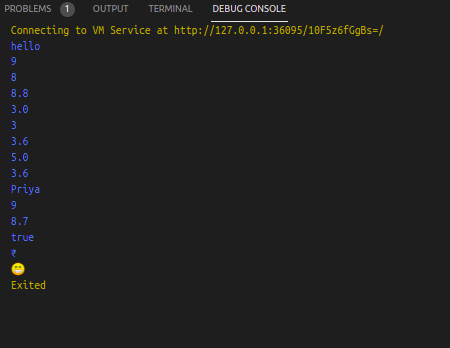
\includegraphics{dart/Output1.png}\\[0.5cm]

\subsection{tostring function, Runtimetype, Initialisation before Use Principale and using ? operator }
\lstinputlisting[language=C,style=mystyle, label=dart/Session1.dart]{dart/Session2.dart}
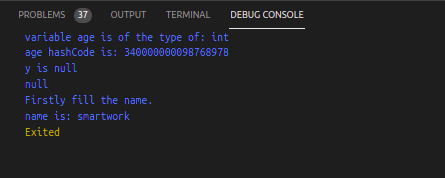
\includegraphics[width=16cm]{dart/initialisationOutput.png}\\[0.5cm]
\subsection{final and const}Assignment1CovidCasesTabularform.dart
\lstinputlisting[language=C,style=mystyle, label=dart/Session1.dart]{dart/Session2final_const.dart}
\subsection{Difference between exit and return \& Named parameters}
\lstinputlisting[language=C,style=mystyle, label=dart/Session5.dart]{dart/Session5.dart}
\subsection{Abstract Class Real Life Example}
\lstinputlisting[language=C,style=mystyle, label=dart/Session7.dart]{dart/Session7.dart}
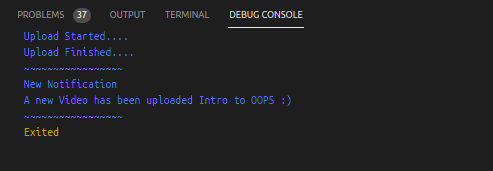
\includegraphics[width=16cm]{dart/abstract.png}\\[0.5cm]
\subsection{Use of 'dart:math' and generate random string}
\lstinputlisting[language=C,style=mystyle, label=dart/stringrandom.dart]{dart/stringrandom.dart}
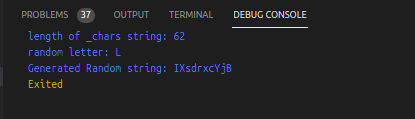
\includegraphics[width=16cm]{dart/randomgeneratestring.png}\\[0.5cm]
\section{Assignment}
\subsection{A Program For Water Bottle Sensor using basic variables and control function}
\lstinputlisting[language=C,style=mystyle, label=dart/Session1.dart]{dart/Session1HW.dart}
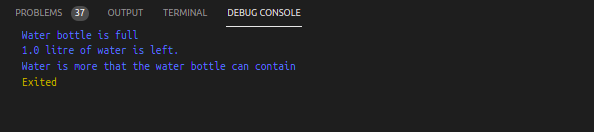
\includegraphics[width=16cm]{dart/waterbottleOutput.png}\\[0.5cm]
\subsection{A Program to sort the covid cases according to the Active, Confirmed, Recovered, Deceased and Tested}
\lstinputlisting[language=C,style=mystyle, label=dart/Assignment1CovidCasesTabularformdart]{dart/Assignment1CovidCasesTabularform.dart}
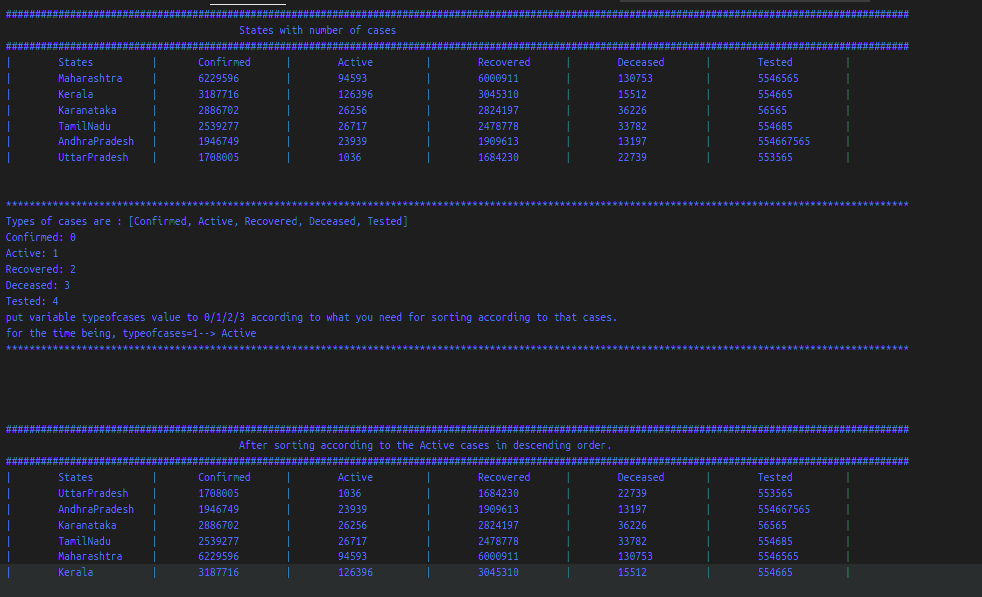
\includegraphics[width=16cm]{dart/covidcases.png}\\[0.5cm]
\subsection{A Program for small case study of website makemytrip using inheritance and classes concept}
\lstinputlisting[language=C,style=mystyle, label=dart/makemytripdart]{dart/makemytrip.dart}
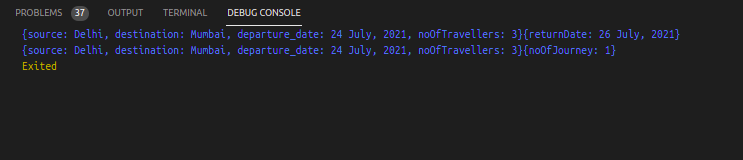
\includegraphics[width=16cm]{dart/makemytrip.png}\\[0.5cm]